%%% exemplo de utilização da classe ita
%%%
%%%   por        fábio fagundes silveira   -  ffs [at] ita [dot] br
%%%              benedito c. o. maciel     -  bcmaciel [at] ita [dot] br
%%%              giovani volnei meinertz   -  giovani [at] ita [dot] br
%%%    	         hudson alberto bode       -  bode [at] ita [dot]br
%%%    	         p. i. braga de queiroz    -  pi [at] ita [dot] br
%%%    	         jorge a. b. gripp         -  gripp [at] ita [dot] br
%%%    	         juliano monte-mor         -  jamontemor [at] yahoo [dot] com [dot] br
%%%    	         tarcisio a. b. gripp      -  tarcisio.gripp [at] gmail [dot] com
%%%
%%%   versão para overleaf:
%%%   por           alejandro a. rios cruz - aarc.88@gmail.com
%%%                 saulo gómez            - sagomezs@unal.edu.co
%%%  importante: o texto contido neste exemplo nao significa absolutamente nada.  :-)
%%%              o intuito aqui eh demonstrar os comandos criados na classe e suas
%%%              respectivas utilizacoes.
%%%
%%%  tese.tex  2016-08-25
%%%  $headurl: http://www.apgita.org.br/apgita/teses-e-latex.php $
%%%
%%% italus
%%% instituto tecnológico de aeronáutica --- ita, sao jose dos campos, brasil
%%%                   http://groups.yahoo.com/group/italus/
%%% discussion list: italus {at} yahoogroups.com
%%%
%++++++++++++++++++++++++++++++++++++++++++++++++++++++++++++++++++++++++++++++
% para alterar o tipo de documento, preencher a linha abaixo \documentclass[?]{?}
%   \documentclass[tg]{ita}			= trabalho de graduacao
%   \documentclass[tgfem]{ita}	= para engenheiras
%   								msc     		= dissertacao de mestrado
%   								mscfem   		= para mestras
%   								dsc      		= tese de doutorado
%   								dscfem   		= para doutoras
%   								quali    		= exame de qualificacao
%   								qualifem 		= exame de qualificacao para doutoras
% para 'draft version'/'versao preliminar' com data no rodape, adicionar 'dv':
%   \documentclass[dsc, dv]{ita}
% para trabalhos em inglês, adicionar 'eng':
%   \documentclass[dsc, eng]{ita}
%		\documentclass[dsc, eng, dv]{ita}
%++++++++++++++++++++++++++++++++++++++++++++++++++++++++++++++++++++++++++++++
\documentclass[tg]{ita}    % ita.cls based on standard book.cls
% quando alterar a classe, por exemplo de [msc] para [msc, eng]) rode mais uma vez o botão build output caso haja erro
\usepackage{ae}
\usepackage{graphicx}
\usepackage{epsfig}
\usepackage{amsmath}
\usepackage{amssymb}
\usepackage{subfig}
\usepackage{multirow}
\usepackage{float}
\usepackage{amsthm}
\usepackage{url}         % formats url addresses properly
\usepackage{appendix}    % allows appendix section to be included
\usepackage{lscape}      % allows a page to be rendered in landscape mode
\usepackage{multicol}    % allows text in multi columns
\usepackage{cancel}      % needed to show canceled terms in equations
\usepackage{lettrine}
\usepackage{float}
\usepackage{placeins}
\usepackage[outputdir=latex.out]{minted}
\usepackage{prettyref}

\renewcommand\listingscaption{Código}
\newcommand{\Baker}{\textit{Baker}}

\newrefformat{anex}{Anexo~\ref{#1}}
\newrefformat{cap}{Capítulo~\ref{#1}}
\newrefformat{fig}{Figura~\ref{#1}}
\newrefformat{lst}{Código~\ref{#1}}
\newrefformat{tbl}{Tabela~\ref{#1}}

% Make ref autocomplete work.
\newcommand{\cref}[1]{\prettyref{#1}}

\usemintedstyle{friendly}

%HHHHHHHHHHHHHHHHHHHHHHHHHHHHHHHHHHHHHHHHHHHHHHHHHHHHHHHHHHHHHHHHHHHHHHHHHHHHHHHHHHHHHHHHHHHHHHHHHHHHHHHHHHHH
%\usepackage{subfigure}
%\usepackage{subfigmat}
%PACOTEFIGURAS_SE _ERRADO_ESXCLUIR_ACIMA
\usepackage{booktabs}
%PACOTETABELAS_SE _ERRADO_ESXCLUIR_ACIMA
%HHHHHHHHHHHHHHHHHHHHHHHHHHHHHHHHHHHHHHHHHHHHHHHHHHHHHHHHHHHHHHHHHHHHHHHHHHHHHHHHHHHHHHHHHHHHHHHHHHHHHHHHHHHH

%++++++++++++++++++++++++++++++++++++++++++++++++++++++++++++++++++++++++++++++
% Espaçamento padrão de todo o documento
%++++++++++++++++++++++++++++++++++++++++++++++++++++++++++++++++++++++++++++++
\onehalfspacing

%singlespacing Para um espaçamento simples
%onehalfspacing Para um espaçamento de 1,5
%doublespacing Para um espaçamento duplo

%++++++++++++++++++++++++++++++++++++++++++++++++++++++++++++++++++++++++++++++
% Identificacoes (se o trabalho for em inglês, insira os dados em inglês)
% Para entradas abreviadas de Professora (Profa.) em português escreva: Prof$^\textnormal{a}$.
%++++++++++++++++++++++++++++++++++++++++++++++++++++++++++++++++++++++++++++++
\course{Engenharia da Computação}

% Autor do trabalho: Nome Sobrenome
\authorgender{masc}
\author{Luis Cláudio Magalhães de}{Holanda}
\itaauthoraddress{Rua Engenheiro Prudente Merieles de Morais, 813, apto 806}{12.243-750}{São José dos Campos--SP}

% Titulo da Tese/Dissertação
\title{Aplicação de Model Driven Development para o aumento de eficiência de um time de desenvolvimento e do serviço Web construído}

% Orientador
\advisorgender{masc}
\advisor{Prof.~Dr.}{Fábio Carneiro Mokarzel}{ITA}

% Coorientador
\coadvisorgender{masc}
\coadvisor{Prof.~Dr.}{Inaldo Capistrano Costa}{ITA}

%Coordenador do curso no caso de TG
\bosscoursegender{masc}
\bosscourse{Prof.~Dr.}{Marcos Ricardo O. de A. Máximo}

% Palavras-Chaves informadas pela Biblioteca -> utilizada na CIP
%\kwcip{Cupim}

% Data da defesa (mês em maiúsculo, se trabalho em inglês, e minúsculo se trabalho em português)
\date{16}{novembro}{2021}

% Número CDU - (somente para TG)
\cdu{XXX.XX}

% Glossario
\makeglossary
\frontmatter

\begin{document}
% Folha de Rosto e Capa para o caso do TG
\maketitle

% Dedicatoria: Nao esqueca essa secao  ... :-)
\begin{itadedication}
Aos amigos da Graduação e Pós-Graduação do ITA por motivarem tanto a criação deste template pelo Fábio Fagundes Silveira quanto por motivarem a mim e outras pessoas a atualizarem e aprimorarem este excelente trabalho.
\end{itadedication}

% Agradecimentos
\begin{itathanks}
Agradeço meus pais, que sempre me apoiaram no caminho que quis seguir, minha irmã
e aos meus amigos, por todo o apoio emocional e moral.

Agradeço também a todos os professores que, de uma forma ou de outra, contribuiram
para o meu desenvolvimento intelectual que me permitiu produzir esse trabalho.

Por fim, agradeço ao time da TerraMagna, que abriu espaço para o desenvolvimento desse
trabalho durante o meu expediente e forneceu insumos para que realizasse os experimentos
necessários.

\end{itathanks}

% Epígrafe
\thispagestyle{empty}
\ifhyperref\pdfbookmark[0]{\nameepigraphe}{epigrafe}\fi
\begin{flushright}
\begin{spacing}{1}
\mbox{}\vfill
{\sffamily\itshape
``Doing the same thing repeatedly, and expecting \\
different results is the definition of insanity''\\}
--- \textsc{Albert Einstein}

\end{spacing}
\end{flushright}

% Resumo
\begin{abstract}
\noindent
Sistemas Web apresentam um grau de complexidade bastante diversificado, variando desde
um sistema comercial de um mercado de bairro até o sistema completo de uma multi-nacional
em escala global. Para simplificar o desenvolvimento desses sistemas, diversas ferramentas
foram desenvolvidas.

Este trabalho apresenta um novo modelo de gerador de APIs, com o objetivo de solucionar
problemas que ferramentas atuais apresentam. Esses problemas são relacionados a baixa
integração com outras ferramentas de desenvolvimento, como Object-Relational Mappings
(ORMs) e validadores. Mostramos também que o uso de um gerador que integre eficientemente
com o restante do ecossistema pode resultar em grandes ganhos de eficiência para o time de
desenvolvimento, além de abrir portas para o uso de outras ferramentas que não seriam possíveis
sem ele. Uma motivação para esse trabalho é a busca do aumento de eficiência e automação dentro
do processo de desenvolvimento e a redução na incidência de defeitos em sistemas complexos.

\end{abstract}

% Abstract
\begin{englishabstract}
\noindent
This work presents a new model of API generator, intending to solve problems that
current solutions have. These problems are related to low integration with other
development tools such as ORMs and validators. We also show that the use of a
generator integrating effectively with the rest of the ecosystem can result in
significant efficiency gains for a development team and open doors for the use of
other tools that would not be possible without it. One motivation for this work
is to search for increased efficiency and automation within the development process
and reduce defects in complex systems.

\end{englishabstract}

% Lista de figuras
\listoffigures %opcional

% Lista de tabelas
\listoftables %opcional

% Lista de abreviaturas
\listofabbreviations
\begin{longtable}{ll}
  API & \textit{Application Programming Interface} \\
  IDL & \textit{Interface Definition Language} \\
  ORM & \textit{Object-Relational Mapping} \\
\end{longtable}

 %opcional

% Lista de simbolos
\listofsymbol
\begin{longtable}{ll}
\end{longtable}

 %opcional

% Sumario
\tableofcontents


\mainmatter
% Os capitulos comecam aqui

\chapter{Introdução}\label{cap:introduction}
\section{Contexto}

Desenvolvimento de aplicações Web apresenta um variado nível de dificuldade e
complexidade: podem variar desde um simples serviço com poucas operações até
um complexo sistema com dezenas (ou centenas) de serviços interligados de maneira
arbitrária com centenas ou milhares de operações.

Nesse contexto, diversas ferramentas foram desenvolvidas para tentar facilitar
e simplificar o desenvolvimento desses sistemas: geradores de APIs e \textit{object-relational
mapping} (ORMs) são exemplos de ferramentas que caem nessa categoria.

\section{\textit{Interface Definition Languages}}

APIs são normalmente especificadas em \textit{Interface Definition Languages}
(IDLs). Essas linguagens possuem construções que facilitam o desenvolvimento de uma
especificação, em relação a operações, entradas, saídas e erros. Qual é usada
depende do tipo de API está sendo construída, alguns exemplos são:

\begin{itemize}
\item
  \textit{Web Service Description Language} \cite{wsdl:spec}: usada para
    definir APIs que usam o protocolo SOAP. É uma linguagem baseada em XML.
    Um exemplo de um arquivo WSDL é apresentado em \cref{anex:wsdl-example}.
\item
  \textit{OpenAPI} \cite{openapi:spec}: comumente usada para definir APIs que usam
    o protocolo HTTP \cite{rfc2616}, informalmente chamadas de \textit{"Restful APIs"}
    em referência ao conceito de REST definido em \cite{10.5555/932295}. É uma linguagem
    baseada em YAML. Um exemplo de um arquivo OpenAPI é apresentado em \cref{anex:openapi-example}.
\item
  \textit{Protocol Buffers} \cite{googl:protobuf}: usada para definir APIs que usam
    o protocolo gRPC \cite{googl:grpc}. O nome se refere tanto à IDL usada para a
    especificação quanto para ao formato binário usado para transmitir as mensagens.
    Um exemplo de um arquivo em Protocol Buffers é apresentado em \cref{anex:protobuf-example}.
\end{itemize}

Existem diversas vantagens em usar uma IDL, entre elas:

\begin{enumerate}
\item
  A comunicação entre diferentes times (possivelmente em diferente organizações) que
  precisam interagir via API é mais simples, já que todos os detalhes de interface
  estão especificados em um formato padrão.
\item
  Pro esse motivo, é muito mais simples construir ferramentas de análise sobre a
  especificação, como geradores de código, validadores, ferramentas de teste, etc.
\end{enumerate}

\section{Geradores de APIs}

Geradores de APIs são ferramentas que, via uma especificação de uma API, conseguem
produzir código-fonte em uma linguagem de programação tanto para realizar requisições
a essa API, quanto para gerar uma base para a implementação da API em si.
O código gerado em ambos os casos contém tanto métodos para as operações suportadas
pela API quanto as estruturas de dados necessárias para interfacear com as mensagens
a serem transmitidas.

Existem diversas vantagens em usar um gerador de API, entre elas:

\begin{enumerate}
\item
  Como toda a parte dos modelos são geradas, servidor ou cliente, há uma significativa
  redução no volume de linhas de código-fonte do sistema, reduzindo a possibilidade
  de defeitos \cite{5010260} e facilitando o entendimento do projeto por novos
  desenvolvedores.
\item
  Como o código é gerado a partir da especificação, sabemos que a implementação
  vai estar de acordo com a interface especificada, permitindo que o programador
  foque em implementar a lógica de cada operação, otimizando o uso do tempo. No
  caso de consumidores, eles poupam o trabalho de ter que implementar um código
  de integração com a API, que pode conter erros e ser difícil de manter,
  principalmente com relação a mudanças e adições na API.
\item
  O código gerado abstrai toda a camada de comunicação e rede, tanto do servidor
  quanto do cliente, facilitando o entendimento do código que o programador precisa
  implementar.
\end{enumerate}

Existem diversos exemplos de geradores de APIs, alguns são \cite{openapi:gen} e
\cite{googl:protobuf}.

\section{ORMs}

Da mesma forma que IDLs e geradores tentam facilitar o desenvolvimento da
\textit{interface} de uma API, ORMs tentam facilitar a integração do código da
API com o banco de dados usado (seja ele SQL ou NoSQL). Elas são bibliotecas que
abstraem a execução de operações no banco de dados em uma interface amigável para
a linguagem de programação usada. Por esse motivo, ORM é específica para a linguagem
de programação em que ela foi implementada, e normalmente também é específica para
um banco ou conjunto de bancos.

ORMs normalmente funcionam via anotações e interfaces que o programador precisa
adicionar ou implementar no código-fonte dos modelos. Essas anotações servem para,
por exemplo, mapear o modelo a uma tabela, um campo a uma coluna, ou uma relação
com outro modelo (1-1, 1-muitos ou muitos-muitos).

Um exemplo em Python usando a ORM \texttt{sqlalchemy} é \cref{lst:sqlalchemy-example}.

\begin{listing}[ht]
\begin{minted}{python}
from sqlalchemy import Column, DateTime, String, Integer, ForeignKey, func
from sqlalchemy.orm import relationship, backref
from sqlalchemy.ext.declarative import declarative_base


Base = declarative_base()


class Department(Base):
    __tablename__ = 'department'
    id = Column(Integer, primary_key=True)
    name = Column(String)


class Employee(Base):
    __tablename__ = 'employee'
    id = Column(Integer, primary_key=True)
    name = Column(String)
    # Use default=func.now() to set the default hiring time
    # of an Employee to be the current time when an
    # Employee record was created
    hired_on = Column(DateTime, default=func.now())
    department_id = Column(Integer, ForeignKey('department.id'))
    # Use cascade='delete,all' to propagate the deletion of a Department
    # onto its Employees
    department = relationship(
        Department,
        backref=backref('employees',
                         uselist=True,
                         cascade='delete,all'))

\end{minted}
\caption{Exemplo de código usando \texttt{sqlalchemy}}
\label{lst:sqlalchemy-example}
\end{listing}

ORMs são populares pois simplificam o trabalho do desenvolvedor ao automatizar muitas
operações que são comumente realizadas no banco, e por prover uma DSL caso seja
necessário fazer algo mais complexo. Dependendo da linguagem, essas funcionalidades
podem ser validadas em tempo de compilação, previnindo defeitos.

\section{Problema}

Apesar de serem ferramentas muito populares, geradores de APIs e ORMs não integram
bem. O primeiro costuma focar na \textit{interface de comunicação}, não prestando
atenção a detalhes de implementação. Além disso, dado o grande número de ORMs
presente para cada linguagem, e também as diversas formas de se gerar a interface
de comunicação, geradores convencionais não conseguiriam adicionar suporte para
todas as combinações possíveis.

Outro problema em como os geradores são implementados hoje é que eles possuem
suporte limitado a extensões externas ao código-fonte. Dependendo do gerador
utilizado, é necessário implementar um \textit{novo gerador}, o que gera um grande
custo operacional. Alguns exemplos de modificações possíveis:

\begin{itemize}
\item
  Geração automática de testes para as operações \cite{9159071}.
\item
  Validação automática de propriedades das mensagens \cite{envoy:protoc-gen-validate}.
\item
  Integração com ORMs ou outras bibliotecas.
\end{itemize}

Devido a esses problemas, muitas organizações deixam de usar essas ferramentas e os
programadores precisam implementar manualmente códigos que poderiam ser gerados.
Isso aumenta a chance de erros ocorrerem durante a implementação, e o resultado divergir
da especificação. Além disso, diminui a eficiência do time, pois há mais tarefas a
serem realizadas.

Avaliando as tarefas realizadas pelo time de engenharia de uma organização durante o
ano de 2020, foi possível identificar que pelos menos 30\% das tarefas realizadas
eram relacionadas a implementação de modelos, integração com ORMs e com a camada
de comunicação da API. Além disso, dentro desses 30\%, ocorreram diversas vezes tarefas
extras relacionadas com ajustes da implementação para que essa seguisse a especificação.

Na tentativa de solucionar esse problema, esse trabalho propõe um novo modelo de
gerador de APIs, que pode ser extendido para suportar qualquer linguagem ou funcionalidade
nova sem a necessidade de modificar o código-fonte.

Esse trabalho é estruturado como se segue. \cref{cap:past-works} faz uma análise
de trabalhos anteriores. \cref{cap:proposal} apresenta, de forma detalhada, o que
foi construído e a metodologia de análise.


\chapter{Trabalhos Anteriores}\label{cap:past-works}
% TODO: maybe talk about LLVM here?

Durante o desenvolvimento desse trabalho, analisamos diversos trabalhos já publicados
relacionados a geradores de APIs, e extensões a IDLs.

\cite{openapi:gen} apresenta uma vasta gama de geradores baseados na IDL OpenAPI. Até
a presente data, apresenta 66 geradores de clientes para 33 linguagens e 41 geradores
de servidores para 16 linguagens. Esse é o principal programa utilizado para gerar
código em projetos que usam OpenAPI para especificação de suas APIs.

Analisando o código-fonte e documentação do projeto, chegamos às seguintes conclusões:

\begin{itemize}
\item
  Os geradores funcionam com base em um modelo genérico baseado em OpenAPI. O processo
  de geração ocorre da seguinte maneira:

  \begin{enumerate}
  \item
    O programa lê a especificação OpenAPI e a transforma no modelo genérico.
  \item
    A classe do gerador modifica esse modelo da forma que precisar, possivelmente
    adicionando propriedades específicas para ele.
  \item
    O programa envia o modelo final para um processador de \textit{templates}, que
    carrega os templates do gerador específico e os renderiza. O resultado dessa
    etapa é o código final.
  \end{enumerate}

  Esse fato pode acabar por limitar a expressividade do gerador, pois o modelo
  OpenAPI não é capaz de expressar, de forma simples, todos os detalhes envolvidos
  em uma linguagem de programação.
\item
  Apesar de ser possível criar um novo gerador customizado, por exemplo, para uma
  linguagem que o projeto não suporte, sem a necessidade de modificar o programa
  em si, os geradores são estruturas monolíticas. Não é possível implementar uma
  funcionalidade nova, e.g. um novo processo de validação, que possa ser usado por
  todos os geradores. Isso limita significativamente a extensibilidade do projeto,
  além de aumentar a carga operacional nessas situações.
\end{itemize}

\cite{googl:protobuf} é o compilador de Protocol Buffers. Ele apresenta uma estrutura
bastante interessante em questão de extensibilidade: o sistema de \textit{plugins}.
Um \textit{plugin} é um programa que recebe uma mensagem \texttt{CodeGeneratorRequest}
como entrada e escreve na saída uma mensagem \texttt{CodeGeneratorResponse}. As
definições dessas duas mensagens são apresentadas em \cref{lst:code-gen-req} e
\cref{lst:code-gen-res}, respectivamente.

\begin{listing}[ht]
\caption{Especificação de \texttt{CodeGeneratorRequest}}
\label{lst:code-gen-req}
\begin{minted}{protobuf}
message CodeGeneratorRequest {
  repeated string file_to_generate = 1;

  optional string parameter = 2;

  repeated FileDescriptorProto proto_file = 15;

  optional Version compiler_version = 3;
}
\end{minted}
\end{listing}

\begin{listing}[ht]
\caption{Especificação de \texttt{CodeGeneratorResponse}}
\label{lst:code-gen-res}
\begin{minted}{protobuf}
message CodeGeneratorResponse {
  optional string error = 1;

  message File {
    optional string name = 1;

    optional string insertion_point = 2;

    optional string content = 15;
  }

  repeated File file = 15;
}
\end{minted}
\end{listing}

Esse sistema é interessante por dois fatores:

\begin{itemize}
\item
  É muito simples adicionar suporte a uma nova linguagem, precisamos apenas
  implementar um \textit{plugin}. Ponto em comum com o trabalho anterior.
\item
  Usando o campo \texttt{file.insertion\_point}, é possível injetar conteúdo
  de um gerador em outro. O segundo gerador pode adicionar esses pontos no
  arquivo gerado por ele, permitindo que outros geradores modifiquem o resultado
  final.

  Isso soluciona, em parte, o problema de adicionar novas funcionalidades em
  um gerador presente em \cite{openapi:gen}. Dois problemas ainda persistem:

  \begin{enumerate}
  \item
    Estamos limitados aos pontos de inserção disponibilizados pelo gerador, o
    que pode variar de uma linguagem para outra. O quão grave é esse problema
    depende do que se quer fazer com o \textit{plugin} e qual é a linguagem objeto.
  \item
    O sistema trabalha em termos de texto (campo \texttt{file.content}). Isso
    limita o quão genérico nossa funcionalidade pode ser, e.g. um \textit{plugin} de
    validação poderia ser genérico caso o resultado fosse mais estruturado.

    Um exemplo de plugin que poderia ser genérico é \cite{envoy:protoc-gen-validate},
    que provê uma extensão para diversas validações. Hoje, ela é limitada para
    as linguagens Go, C++ e Java. Caso o resultado fosse mais estruturado, seria
    possível implementar tal funcionalidade de forma genérica para uma grande
    quantidade de linguagens.
  \end{enumerate}
\end{itemize}

\cite{9159071} se propõe a resolver um problema diferente dos trabalhos anteriores:
ele gera testes baseado em \textit{Property Based Testing} \cite{10.1145/351240.351266}
a partir de especificações OpenAPI que validam que as respostas da API seguem as
propriedades e formatos especificados. O programa é capaz de gerar esses testes
sem a necessidade de nenhuma extensão a especificação.

\cite{sferruzza:hal-01868498} propõe extensões e um gerador para OpenAPI que é
capaz de modelar como uma operação é implementada. O trabalho cria o conceito de
\textit{componentes atômicos e compostos}: componentes atômicos recebem parâmetros
e podem gerar novos valores e componentes compostos fazem a composição de diversos
componentes para definir uma dada lógica. O programa então é capaz de validar que
as definições e uso dos componentes são válidas, tanto em questão de todas as
variáveis estarem disponíveis quanto que os tipos estão corretos. O gerador é capaz
de gerar código que define esses componentes.

Por fim, \cite{r2c:semgrep} é uma ferramenta de análise estática que suporta uma
quantidade impressionante de linguagens. O diferencial dessa ferramenta é que
o usuário pode criar novas regras de análise utilizando uma DSL implementada sobre
YAML, permitindo que a mesma regra seja aplicada em diversas linguagens. Isso
é possível pois todas as linguagens que ela suporta são convertidas para
\textit{uma mesma linguagem intermediária} antes das regras serem aplicadas. Essa
funcionalidade é similar a situação em que queremos implementar uma funcionalidade
no nosso gerador de forma independente da linguagem objeto.


\chapter{Projeto}\label{cap:project}
A hipótese base deste trabalho é que, baseado nos projetos mencionados anteriormente,
é possível implementar um novo modelo de gerador que seja muito mais extensível, amigável
e que consiga aplicar funcionalidades mais genéricas. Além disso, outra hipótese
é que, com base nessa extensibilidade, conseguimos aumentar de forma considerável a
eficiência de um time de desenvolvimento, utilizando o gerador para automatizar
trabalhos repetitivos.

\section{\Baker{}}

O projeto desenvolvido nesse trabalho, e seu resultado principal, é o programa \Baker{}
\cite{baker}, uma plataforma para desenvolvimento de geradores de código componentizáveis.
O projeto usa como base a IDL Protocol Buffers, por ser mais amigável ao desenvolvedor e
por possuir um ecossitema maduro de ferramentas de análise e de suporte.

Com foco em extensibilidade, o projeto tenta realizar o minímo de escolhas que impeçam ou
dificultem autores de construir geradores na plataforma. Além disso, as interfaces entre o
programa e os geradores foram pensadas para facilitar a construção programática e estruturada
do código, ao invés de ser baseada em texto ou processador de \textit{templates}.

O programa separa geradores em dois tipos, cada um responsável por parte do fluxo de geração:

\begin{itemize}
\item \textit{Layers}: Programas responsáveis por gerar, a partir das estruturas construídas
  a partir dos arquivos fonte do usuário, fragmentos de código na linguagem intermediária (IR)
  do projeto. Cada \textit{layer} é responsável por gerar apenas parte do resultado final, os
  resultados de cada uma são combinados para formarem a estrutura intermediária final.
\item \textit{Codegens}: Programa responsável por, a partir da estrutura em IR gerada por todas
  as \textit{layers}, gerar o código final na linguagem objeto.
\end{itemize}

A escolha em separar os geradores nessas duas categorias é devida aos seguintes fatores:

\begin{itemize}
\item Ao limitarmos a lógica de tradução IR $\rightarrow$ linguagem objeto aos \textit{codegens},
  e que esses possuam apenas essa lógica, permitimos que \textit{layers} se preocupem apenas com
  \textit{qual} código deve ser gerado, e não em \textit{como};
\item Pelo mesmo motivo, diminuímos o custo de construção de novas \textit{layers}, já que o
  trabalho que precisam realizar é menor. Além disso, simplificamos a troca de uma \textit{layer}
  por outra que gere uma integração com a mesma biblioteca de uma forma diferente, aumentando o
  grau de customização pelos usuários;
\item O fato de combinarmos os resultados de todas as \textit{layers} de forma estruturada e clara
  permite que cada uma seja responsável por apenas parte do código final, sem depender que códigos
  anteriores tenham gerado os \textit{entrypoints} necessários (quando comparado com
  \textit{plugins} de \cite{googl:protobuf});
\item O foco na construção programática do código diminui a barreira de entrada para novos
  desenvolvedores, já que técnicas padrão de desenvolvimento de software podem ser aplicadas sem
  dificuldades, pois todos os dados que o desenvolvedor lida são estruturados.
\end{itemize}

\subsection{Representação Intermediária (IR)}

A IR utilizada pelo programa para armazenar o código a ser gerado é, na realidade, apenas um
conjunto de estruturas definidas em Protocol Buffers, não possuindo representação textual e
muitas dessas estruturas não possuem comportamento definidos. Essas estruturas possuem apenas
o mínimo de especificação para que autores de \textit{layers} e \textit{codegens} sejam capazes
de mapear cada estrutura para um análogo na linguagem objeto. Essa escolha é feita para evitar
que \Baker{} limite o que pode ser gerado.

Como veremos, o fato da IR ser definida em Protocol Buffers possibilita que geradores sejam
construidos em qualquer linguagem que possua suporte ao formato.

A IR é estruturada da seguinte maneira:

\begin{itemize}
\item Cada arquivo fonte é ligado a uma (ou mais) \texttt{IrFile}s.
\item Cada \texttt{IrFile} contém um \texttt{Namespace} raiz.
\item \texttt{Namespace}s são responsáveis por armazenar definições a serem geradas, que podem ser:
  funções, tipos (que podem ser \textit{record types}, e.g. \texttt{struct}s, ou \textit{sum types},
  e.g. \texttt{enum}s), funções, interfaces, constantes ou mesmo outros \texttt{Namespace}s. Podemos
  pensar em um \texttt{Namespace} dentro de outro \texttt{Namespace} como uma forma de expressar
  submódulos, mas também pode ser usado para declarar estruturas dentro de outras (e.g. uma classe
  dentro de outra).
\item Declarações de tipos contém tanto a estrutura do tipo em si (propriedades ou membros), como
  também atributos aplicados ao tipo, documentação e uma série de \texttt{ImplBlock}s.
\item \texttt{ImplBlock} é usado para definir uma série de implementações para um tipo específico,
  como implementar uma certa interface, adicionar métodos, etc. Em cada bloco, uma série de restrições
  podem ser adicionadas, e.g. limitar genéricos a obedecerem uma dada interface. A separação em
  uma série de blocos simplifica a construção de \textit{layers} e também leva em conta que
  existem linguagens com essa funcionalidade.
\end{itemize}


\subsection{Processo de Geração}

Com essas definições em mãos, o fluxo do programa é:

\begin{enumerate}
\item A partir dos arquivos fonte passados, processamos pacotes, mensagens, serviços e enums
  definidos na origem. Esse processo requer identificar corretamente, a partir do escopo atual,
  a qual estrutura cada campo se refere. No final desse processo, o grafo contém a lista
  normalizada das estruturas declaradas. Uma lista não exaustiva do processo de normalização é:

  \begin{itemize}
  \item Todos os nomes das estruturas são convertidos para nomes absolutos (pacote + escopo + nome),
    e.g. \texttt{Foo} é convertido para \texttt{foo.v1.Foo};
  \item Linhas de documentação são combinadas em um único texto;
  \item Referências a nomes de estruturas são convertidos para os identificadores das mesmas no
    grafo. Permitindo que sejam facilmente buscadas;
  \item Convertemos diversas estruturas padrões de Protocol Buffers para tipo normalizados, que
    podem ser usados mais facilmente por \textit{layers}, e.g. o tipo \texttt{google.protobuf.Timestamp}
    é convertido para o tipo normalizado \texttt{TIMESTAMP}.
  \end{itemize}

  Esse processo é realizado pela entidade denominada \textit{Proto Loader}.
\item Enviamos o grafo gerado para cada uma das \textit{layers}, em ordem recebida pelo programa.
  Cada uma dessas responde com um pedaço de código na IR do projeto.
\item Todas as respostas em IR são combinadas em uma única estrutura. O processo de combinação é
  uma possível área de melhoria, sendo feito, no momento de escrita, as seguintes combinações:

  \begin{itemize}
  \item Para cada \textit{namespace}, combinamos todas as definições entre duas respostas.
  \item Para definições de tipos com o mesmo nome, caso ambas as definições sejam do mesmo formato:
    \begin{enumerate}
    \item No caso de \textit{record types}, combinamos todas as propriedades em ambas as definições.
      Caso a mesma propriedade exista em ambas, a visibilidade é modificada para a mais permissiva e
      atributos são agrupados.
    \item No caso de \textit{sum types}, agrupamos apenas atributos em membros que existam em ambas
      as definições. A possibilidade de se adicionar novos membros a um \textit{sum type} é uma questão
      em aberto, devido a facilidade de gerar códigos objeto invalidos.
    \end{enumerate}
  \item Outras definições são apenas agrupadas.
  \end{itemize}

  Esse processo é realizado pela entidade denominada \textit{IR Merger}.
\item A estrutura final é enviada para o \textit{codegen} final, que fará a conversão para código
  objeto e também \textit{salvará o arquivo final em disco}. O fato do \textit{codegen} fazer a
  escrita em disco é para darmos flexibilidade e permitimos outros tipos de geração, e.g. usar
  a IR para realizar migrações em bancos de dados.
\end{enumerate}

A \cref{fig:baker-data-flow} apresenta um digrama simplificado do fluxo de dados do programa.

\begin{figure}[h]
  \centering
  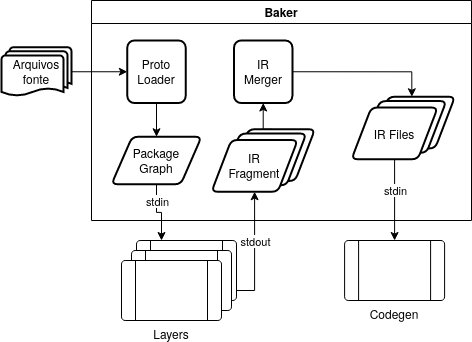
\includegraphics[width=0.8\linewidth]{Imagens/baker-diagram.png}
  \caption{Digrama do Fluxo de Dados do programa}
  \label{fig:baker-data-flow}
\end{figure}

\subsection{Comunicação Entre Programas}

Para permitir que os programas sejam escritos no maior número de linguagens de programação, a comunicação
entre o programa principal, \textit{layers} e \textit{codegens} é feita de forma similar a plugins para
\cite{googl:protobuf}: toda a comunicação é feita via entrada e saída padrão e utilizando Protocol Buffers
como formato. A saída padrão para erros é redirecionada para a saída padrão do programa como um todo, para
facilitar o relato de erros ao usuário.

O uso de Protocol Buffers ao invés de um formato customizado ou até mesmo JSON é devido a:

\begin{itemize}
\item Mantemos o padrão e simplificamos o fluxo.
\item Garante que as estruturas sejam construídas e geradas corretamente.
\item Facilita a manutenção de compatibilidade com \textit{layers} baseadas em versões anteriores
  da ferramenta.
\end{itemize}

\section{Experimento}

Para experimentarmos com a plataforma, identificar pontos de melhoria durante a construção e
servir como base para o experimento de validação, construimos uma série de \textit{layers} e
um \textit{codegen} para a linguagem de programação Rust \cite{rust:site}. Os geradores foram
escolhidos com o objetivo de permitir usuários construirem serviços Web utilizando a plataforma.

\subsection{\textit{Layers} Definidas}

Mantendo a ideia de componentização dos geradores, cada \textit{layer} é responsável por apenas
parte do código gerado: cada uma gera a integração com uma biblioteca específica. Como a troca
de uma \textit{layer} por outra é simples, é possível tomar decisões por padrão sem limitar o
usuário.

\subsubsection{\texttt{rust-types}}

A primeira \textit{layer} desenvolvida, e a primeira que deve ser passada para o programa, é
o gerador responsável por traduzir as mensagems definidas nos arquivos fonte em tipos da linguagem
objeto. Esse deve ser o primeiro programa a ser passado devido as regras de combinação de IR: o
primeiro resultado é aquele que tem prioridade na definição de campos dos tipos.

Um exemplo simples de código gerado é apresentado pelas listagens \ref{lst-rust-types-proto-src}
e \ref{lst-rust-types-rust-out}, onde uma \textit{struct} em Rust é gerada a partir de uma
\textit{message} em Protocol Buffers. Um ponto a ser comentado é que, apesar de estarmos construindo
um gerador de código, isso não significa que não possamos utilizar mecânicas de geração da própria
linguagem objeto. No nosso exemplo, o uso do atributo \texttt{derive} permite que mais código seja
gerado pelo compilador da linguagem, simplificando o código gerador e facilitando o entendimento
do mesmo pelos desenvolvedores.

\begin{listing}
\begin{minted}{protobuf}
// Response of the [`ListPets`] RPC method.
message ListPetsResponse {
  // A paged array of pets.
  repeated Pet pets = 1;
  // A link to the next page of responses.
  optional string cursor = 2;
}
\end{minted}
\caption{Exemplo de entrada para a \textit{layer} \texttt{rust-types}}
\label{lst-rust-types-proto-src}
\end{listing}

\begin{listing}
\begin{minted}{rust}
/// Response of the [`ListPets`] RPC method.
#[derive(Clone, Debug, Default, PartialEq)]
struct ListPetsResponse {
    /// A paged array of pets
    pub pets: Vec<Pet>,
    /// A link to the next page of responses
    pub cursor: Option<String>
}
\end{minted}
\caption{Exemplo de saida da \textit{layer} \texttt{rust-types}}
\label{lst-rust-types-rust-out}
\end{listing}

Um exemplo mais complexo é apresentado nas listagens \ref{lst-rust-types-cplx-proto-src} e
\ref{lst-rust-types-cplx-rust-out}. Nesse exemplo, mostramos o código gerado para um \texttt{enum}
e uma mensagem com campo \texttt{oneof}. No caso do \texttt{oneof}, é necessário gerar um
\texttt{enum} adicional que garante que apenas um dos campos do \texttt{oneof} está presente,
ou que nenhum esteja (membro \texttt{NotSet}).

\begin{listing}
\begin{minted}{protobuf}
// Possible formats of content in a Post.
enum ContentFormat {
  // Conventional default.
  UNKNOWN = 0;
  // The post was written in plain text.
  PLAIN_TEXT = 1;
  // The post was written in markdown.
  MARKDOWN = 2;
}

// A user in the service.
message User {
  // ID of the user.
  int64 id = 1;
  // Name of the user.
  string name = 2;

  // Idenfier of the user.
  oneof identifier {
    // The user used an email to identify himself.
    string email = 3;
    // The user used a username to identify himself.
    string username = 4;
  };
}
\end{minted}
\caption{Exemplo Complexo de entrada para a \textit{layer} \texttt{rust-types}}
\label{lst-rust-types-cplx-proto-src}
\end{listing}

\begin{listing}
\begin{minted}{rust}
/// Possible formats of content in a Post.
#[derive(Clone, Copy, Debug, PartialEq, PartialOrd, Eq, Ord, Hash)]
enum ContentFormat {
    /// Conventional default.
    Unknown = 0,
    /// The post was written in plain text.
    PlainText = 1,
    /// The post was written in markdown.
    Markdown = 2,
}

impl Default for ContentFormat {
   fn default() -> Self {
      Self::Unknown
   }
}

/// A user in the service.
struct User {
    /// ID of the user.
    pub id: i64,
    /// Name of the user.
    pub name: String,
    /// Identifier of the user.
    pub identifier: user::Identifier
}

pub mod user {
    /// Idenfier of the user.
    pub enum Identifier {
        /// Default value for the OneOf. Used when no field is set.
        NotSet,
        /// The user used an email to identify himself.
        Email(String),
        /// The user used a username to identify himself.
        Username(String)
    }

    impl Identifier {
        pub fn is_set(&self) -> bool {
            self != &Self::NotSet
        }
    }

    impl Default for Identifier {
        fn default() -> Self {
            Self::NotSet
        }
    }
}
\end{minted}
\caption{Exemplo Complexo de saida da \textit{layer} \texttt{rust-types}}
\label{lst-rust-types-cplx-rust-out}
\end{listing}

\subsubsection{\texttt{rust-serde}}

Outra \textit{layer} definida é aquela que integra o código gerado com a biblioteca
de serialização/deserialização \texttt{serde} \cite{rust:serde}, a biblioteca padrão
para essa funcionalidade. A integração é feita via diversos atributos adicionados a
tipos, campos e membros. Por padrão, os campos são recebidos e enviados em \texttt{camelCase}
e valores de \texttt{enum}s em \texttt{SCREAMING\_SNAKE\_CASE}, mas o \textit{casing}
pode ser escolhido utilizado as opções \texttt{baker.api.*\_name\_case}. Os nomes também
podem ser renomeados com as opções \texttt{baker.api.*\_name}.

\subsubsection{\texttt{rust-diesel}}

Para demonstrar que é possível integrar uma ORM ao código gerado sem dificuldades, uma
\textit{layer} foi construida para integrar a ORM \texttt{diesel} \cite{rust:diesel},
uma ORM para bancos relacionais SQL. Para a integração, atributos, \texttt{ImplBlock}s
e diversas opções são necessários, como pode ser visto nos \cref{anex:blog-spec} e
\cref{anex:blog-codegen}.

O código gerado não somente integra com a biblioteca, mas também fornece uma série de
utilidades para o programador que não são disponibilizadas normalmente, facilitando o
uso do código gerado. Entre essas utilidades, está a criação de um tipo que pode ser
utilizado nos \textit{schemas} das tabelas em colunas que armazenam \texttt{enum}s
(\texttt{ContentFormatSql} no código gerado do \cref{anex:blog-codegen}).

\subsubsection{\texttt{rust-actix}}

Por fim, a última \textit{layer} desenvolvida integra com o \textit{framework} Web
\texttt{actix-web} \cite{rust:actix-web}. A integração se preocupa em mapear
\texttt{service}s definidos nos arquivos fonte em uma interface que o programador
implemente sem se preocupar com detalhes do \textit{framework}. Dessa forma, todos
os detalhes do contrato da API são gerados automaticamente e o desenvolvedor precisa
somente se preocupar com a lógica de cada operação.

Para configurar a integração, opções nos métodos \texttt{rpc} do serviço são adicionadas,
descrevendo a rota de cada operação (junto com quaisquer variáveis de rota) e o método
HTTP necessário. Para cada operação então, é gerado uma função que recebe a requisição
HTTP, monta o objeto parâmetro a operação, chama o método correto da interface e converte
a resposta do método em uma resposta HTTP.

Para montar o serviço no servidor, é provido um método \texttt{configure} na interface,
que é responsável por criar todas as rotas no servidor (\texttt{trait BlobService} no
código gerado do \cref{anex:blog-codegen}).

\subsection{\texttt{rust-codegen}}

O último programa desenvolvido é o \textit{codegen} para a linguagem. Como podemos
implementar o programa na própria linguagem, é possível utilizar tais ferramentas de
análise (e.g. \textit{parser} e ASTs). Com essas ferramentas em mão, implementar o programa
é uma questão de mapear a IR para a AST da linguagem. Por fim, para facilitar a leitura
do arquivo final, o programa também executa um formatador de código no mesmo.


\chapter{Validação}\label{cap:validation}
Para validarmos a viabilidade da solução, o funcionamento dos geradores implementados e
a qualidade do código resultante, um serviço Web simples foi implementado. Esse serviço
implementa um pequeno blog público, em que usuários podem postar mensagens, comentários
e votar em outras postagens. Mantendo a API simples, conseguimos focar melhor no impacto
do código gerado. A especificação da API é apresentada no \cref{anex:blog-spec}.

Em seguida, foi realizada uma pesquisa com alguns desenvolvedores da empresa TerraMagna,
para que esses julguassem a qualidade do código gerado. Por fim, foi feita uma análise de
outras oportunidades de geradores que facilitariam a implementação de serviços no time.

\section{Implementação do Serviço Web}

Na implementação do serviço, o código gerado é responsável por 64.8\% das linhas de código
total da implementação (633 de 976 linhas). O código gerado é apresentado na íntegra no
\cref{anex:blog-codegen}. Dessas 633 linhas:

\begin{itemize}
\item 135 são da integração com o \textit{framework} web;
\item 228 são da integração com a ORM;
\item os 270 restantes são definições de estruturas.
\end{itemize}

O código implementado manualmente é responsável apenas pela regra de negócio da aplicação,
dispensando preocupação com detalhes de interface da API ou diversos detalhes de bancos
de dados.

À medida que a complexidade do serviço aumenta e a quantidade de regras de negócio também,
a porcentagem total do código gerado diminui. Contudo, outras vantagens se mantêm:

\begin{itemize}
\item O programador não precisa se preocupar em implementar as estruturas manualmente com
  base na especificação. Em situações multi-linguagem ou multi-repositórios, garantir que
  as implementações manuais obedeçam o contrato especificado torna-se complexo. Esse tipo
  de situação é muito comum, principalmente durante o processo de evolução da API.
\item Pelo mesmo motivo, testes de contrato não são, em grande parte, necessários, pois o
  serviço foi gerado a partir da especificação. Apenas testes de contrato para erros são
  necessários, caso o time os faça, já que a especificação não declara tais casos.
\item A especificação continua sendo a fonte da verdade: em sistemas complexos, uma grande
  quantidade de APIs são implementadas e disponibilizadas, ter a garantia de que as operações
  especificadas são as que estão disponíveis facilita a entrada de novos desenvolvedores no
  time e o descobrimento das operações pelos clientes.
\end{itemize}

\section{Qualidade do Código Gerado}

Quando apresentados a um gerador de código, um dos fatores que dificultam o uso é a qualidade
do código gerado e o quão complexo ele é. Na situação em que o time decide deixar de utilizar
o gerador, os desenvolvedores devem manter o código que foi gerado, quanto mais complexo este
for, mais difícil é esse processo.

Para validarmos que essa preocupação não afetaria o uso dos geradores implementados, uma
pesquisa qualitativa foi realizada com membros do time de desenvolvimento da TerraMagna com
um variado grau de senioridade. Nessa pesquisa, após apresentados os \cref{anex:blog-spec} e
\cref{anex:blog-codegen}, foram feitas as seguintes perguntas:

\begin{enumerate}
\item Alguma parte do código que deixa claro que ele foi gerado?
\item É possível entender o que o código faz e como ele é usado?
\item Na hipótese que o gerador deixe de ser usado, você acharia complexo limpar o código?
\end{enumerate}

As respostas à pesquisa foram bem similares. O fato dos caminhos serem absolutos deixa claro
que o código foi gerado, pois programadores em geral importam itens específicos ou criam
\textit{aliases} para caminhos extensos. Contudo, o código continua sendo simples de se
entender e usar. Todos os entrevistados declararam que conseguiriam limpar o código sem
grandes dificuldades, principalmente contando com a ajuda de um bom editor de texto. Além
disso, todos também comentaram que prefeririam usar o código gerado para não terem que
escrever códigos repetitivos.

Caminhos absolutos são utilizados na implementação atual dos geradores para evitarem conflitos
com estruturas declaradas na especificação. Uma melhoria futura nos geradores pode utilizar a
lista de estruturas para determinar se um caminho absoluto é necessário ou não. Essa foi a
principal observação e sugestão feita pelos entrevistados.

\section{Oportunidades}

Apesar de os geradores atuais já facilitarem a implementação de serviços Web, é necessário
entender se há oportunidades para outros geradores. A falta de oportunidades mostraria que
o uso de geradores em ambientes \textit{enterprise} é, de fato, limitado.

Analisando o código dos serviços internos da empresa, encontramos as seguintes oportunidades:

\begin{itemize}
\item Suportar outros sistemas de bancos de dados que não utilizam \texttt{diesel}, como
  Firestore \cite{google:megastore}.
\item Suportar a declaração de mensagems para o sistema de mensageria interno da empresa.
\item Permitir a especificação de requisitos de autorização para os métodos \texttt{rpc}
  seguindo o padrão da empresa, e.g. a operação \texttt{CreateFoo} requer a permissão
  \texttt{BAR.FOO.WRITE}.
\item Declarar condições de estabilidade das operações: \textit{alpha}, \textit{beta},
  \textit{internal only}, \textit{external}. Essas condições são importantes para testes
  e evolução das APIs sem impactar clientes.
\item Integração com o sistema de monitoramento e observabilidade automático para as operações.
\end{itemize}

Essas oportunidades são apenas aquelas que impactam a implementação do serviço \textit{per se}.
Diversas outras oportunidades podem existir quando também consideramos que podemos utilizar
as especificações para gerar clientes, como integrações com bibliotecas de armazenamento em
memória (e.g. \textit{React Redux}).

Com essa lista, podemos perceber que existem diversas formas que o projeto implementado pode
simplificar a implementação dos serviços, aumentar a segurança e confiabilidade dos serviços
e também diminuir a carga cognitiva dos desenvolvedores envolvidos no sistema.


\chapter{Conclusão}\label{cap:conclusion}


% REFERENCIAS BIBLIOGRAFICAS
\renewcommand\bibname{\itareferencesnamebabel} %renomear título do capítulo referências
\bibliography{referencias}

\annex
\chapter{Exemplo em WSDL}\label{anex:wsdl-example}
\begin{minted}{xml}
<?xml version="1.0" encoding="UTF-8"?>
<description xmlns="http://www.w3.org/ns/wsdl"
             xmlns:tns="http://www.tmsws.com/wsdl20sample"
             xmlns:whttp="http://schemas.xmlsoap.org/wsdl/http/"
             xmlns:wsoap="http://schemas.xmlsoap.org/wsdl/soap/"
             targetNamespace="http://www.tmsws.com/wsdl20sample">

<documentation>
  This is a sample WSDL 2.0 document.
</documentation>

<!-- Abstract type -->
  <types>
    <xs:schema xmlns:xs="http://www.w3.org/2001/XMLSchema"
               xmlns="http://www.tmsws.com/wsdl20sample"
               targetNamespace="http://www.example.com/wsdl20sample">
     <xs:element name="Error" type="Error"/>
     <xs:element name="Pet" type="Pet"/>
     <xs:element name="Pets" type="Pets"/>
     <xs:element name="NewPet" type="NewPet"/>

     <xs:element name="ListPetsRequest" type="ListPetsRequest"/>
     <xs:element name="ShowPetByIdRequest" type="ShowPetByIdRequest"/>

     <xs:complexType name="Error">
      <xs:attribute name="code" type="xs:int"/>
      <xs:attribute name="message" type="xs:string"/>
     </xs:complexType>
     <xs:complexType name="Pet">
      <xs:attribute name="id" type="xs:int"/>
      <xs:attribute name="name" type="xs:string"/>
      <xs:attribute name="tag" type="xs:string" nillable="true"/>
     </xs:complexType>
     <xs:complexType name="NewPet">
      <xs:attribute name="name" type="xs:string"/>
      <xs:attribute name="tag" type="xs:string" nillable="true"/>
     </xs:complexType>
     <xs:complexType name="Pets">
      <xs:sequence>
        <xs:element minOccurs="0" name="pets" type="tns:Pet"/>
      </xs:sequence>
     </xs:complexType>

     <xs:complexType name="ListPetsRequest">
      <xs:attribute name="limit" type="xs:int" nillable="true"/>
      <xs:attribute name="cursor" type="xs:string" nillable="true"/>
     </xs:complexType>

     <xs:complexType name="ShowPetByIdRequest">
      <xs:attribute name="id" type="xs:int"/>
     </xs:complexType>
    </xs:schema>
  </types>

<!-- Abstract interfaces -->
  <interface name="PetStoreInterface">
    <fault name="Error1" element="tns:Error"/>
    <operation name="ListPets" pattern="http://www.w3.org/ns/wsdl/in-out">
      <input messageLabel="In" element="tns:ListPetsRequest"/>
      <output messageLabel="Out" element="tns:Pets"/>
    </operation>
    <operation name="CreatePet" pattern="http://www.w3.org/ns/wsdl/in-out">
      <input messageLabel="In" element="tns:NewPet"/>
      <output messageLabel="Out" element="tns:Pet"/>
    </operation>
    <operation name="ShowPetById" pattern="http://www.w3.org/ns/wsdl/in-out">
      <input messageLabel="In" element="tns:ShowPetByIdRequest"/>
      <output messageLabel="Out" element="tns:Pet"/>
    </operation>
  </interface>

<!-- Concrete Binding Over HTTP -->
  <binding name="HttpBinding" interface="tns:PetStoreInterface"
           type="http://www.w3.org/ns/wsdl/http">
    <operation ref="tns:ListPets" whttp:method="GET"/>
    <operation ref="tns:CreatePet" whttp:method="POST"/>
    <operation ref="tns:ShowPetById" whttp:method="GET"/>
  </binding>

<!-- Concrete Binding with SOAP-->
  <binding name="SoapBinding" interface="tns:PetStoreInterface"
           type="http://www.w3.org/ns/wsdl/soap"
           wsoap:protocol="http://www.w3.org/2003/05/soap/bindings/HTTP/"
           wsoap:mepDefault="http://www.w3.org/2003/05/soap/mep/request-response">
    <operation ref="tns:Get" />
    <operation ref="tns:CreatePet" />
    <operation ref="tns:ShowPetById" />
  </binding>

<!-- Web Service offering endpoints for both bindings-->
  <service name="PetStoreService" interface="tns:PetStoreInterface">
    <endpoint name="HttpEndpoint"
              binding="tns:HttpBinding"
              address="http://www.example.com/rest/"/>
    <endpoint name="SoapEndpoint"
              binding="tns:SoapBinding"
              address="http://www.example.com/soap/"/>
  </service>
</description>
\end{minted}


\chapter{Exemplo em OpenAPI}\label{anex:openapi-example}
\begin{minted}{yaml}
openapi: "3.0.0"
info:
  version: 1.0.0
  title: Swagger Petstore
  license:
    name: MIT
servers:
  - url: http://petstore.swagger.io/v1
paths:
  /pets:
    get:
      summary: List all pets
      operationId: listPets
      tags:
        - pets
      parameters:
        - name: limit
          in: query
          description: How many items to return at one time (max 100)
          required: false
          schema:
            type: integer
            format: int32
      responses:
        200:
          description: An paged array of pets
          headers:
            x-next:
              description: A link to the next page of responses
              schema:
                type: string
          content:
            application/json:
              schema:
                $ref: "#/components/schemas/Pets"
        default:
          description: unexpected error
          content:
            application/json:
              schema:
                $ref: "#/components/schemas/Error"
    post:
      summary: Create a pet
      operationId: createPets
      tags:
        - pets
      responses:
        201:
          description: Null response
        default:
          description: unexpected error
          content:
            application/json:
              schema:
                $ref: "#/components/schemas/Error"
  /pets/{petId}:
    get:
      summary: Info for a specific pet
      operationId: showPetById
      tags:
        - pets
      parameters:
        - name: petId
          in: path
          required: true
          description: The id of the pet to retrieve
          schema:
            type: string
      responses:
        200:
          description: Expected response to a valid request
          content:
            application/json:
              schema:
                $ref: "#/components/schemas/Pets"
        default:
          description: unexpected error
          content:
            application/json:
              schema:
                $ref: "#/components/schemas/Error"
components:
  schemas:
    Pet:
      required:
        - id
        - name
      properties:
        id:
          type: integer
          format: int64
        name:
          type: string
        tag:
          type: string
    Pets:
      type: array
      items:
        $ref: "#/components/schemas/Pet"
    Error:
      required:
        - code
        - message
      properties:
        code:
          type: integer
          format: int32
        message:
          type: string
\end{minted}


\chapter{Exemplo em Protocol Buffers}\label{anex:protobuf-example}
\begin{minted}{protobuf}
syntax = "proto3";

import "google/protobuf/empty.proto";

package petstore;

// Interface exported by the server.
service PetStoreService {
  // List all pets.
  rpc ListPets(ListPetsRequest) retuns (ListPetsResponse);

  // Create a pet.
  rpc CreatePet(CreatePetRequest) returns (google.protobuf.Empty);

  // Info for a specific pet.
  rpc ShowPetById(ShowPetByIdRequest) returns (Pet);
}

message ListPetsRequest {
  // How many items to return at one time (max 100).
  optional uint32 limit = 1;
  // A link to the page of responses
  optional string cursor = 2;
}

message ListPetsResponse {
  // A paged array of pets
  repeated Pet pets = 1;
  // A link to the next page of responses
  optional string cursor = 2;
}

message CreatePetRequest {
  string name = 2;
  optional string tag = 3;
}

message ShowPetByIdRequest {
  // The id of the pet to retrieve
  uint64 id = 1;
}

message Pet {
  uint64 id = 1;
  string name = 2;
  optional string tag = 3;
}
\end{minted}



\chapter{Especificação API Blog}\label{anex:blog-spec}
\begin{minted}{protobuf}
syntax = "proto3";

package blog.api.v1;

// A service that provide blog functionalities.
service BlobService {
  option (baker.api.default_http_body_encoding) = JSON;

  // List the users in the system.
  rpc ListUsers(ListUsersRequest) returns (ListUsersResponse) {
    option (baker.api.http_path) = "/v1/users";
    option (baker.api.http_method) = GET;
  }

  // List a number of posts in the system.
  rpc ListPosts(ListPostsRequest) returns (ListPostsResponse) {
    option (baker.api.http_path) = "/v1/posts";
    option (baker.api.http_method) = GET;
  }

  // List comments of a given post.
  rpc ListPostComments(ListPostCommentsRequest) returns (ListPostCommentsResponse) {
    option (baker.api.http_path) = "/v1/posts/{post}/comments";
    option (baker.api.http_method) = GET;
  }

  // Create a post in the system.
  rpc CreatePost(CreatePostRequest) returns (Post) {
    option (baker.api.http_path) = "/v1/posts";
    option (baker.api.http_method) = POST;
  }

  // Post a comment.
  rpc PostComment(PostCommentRequest) returns (Post.Comment) {
    option (baker.api.http_path) = "/v1/posts/{comment.post_id}/comments";
    option (baker.api.http_method) = POST;
  }

  // {Dis}Like a post.
  rpc LikePost(LikePostRequest) returns (Post) {
    option (baker.api.http_path) = "/v1/posts/{post}:like";
    option (baker.api.http_method) = POST;
  }
}

// Request for `ListUsers` RPC method.
message ListUsersRequest {}

// Response for `ListUsers` RPC method.
message ListUsersResponse {
  // Users returned for the request.
  repeated User users = 1;
}

// Request for `ListPosts` RPC method.
message ListPostsRequest {
  // Return posts after a given ID.
  optional int64 after = 1;

  // Limit the number of returned posts.
  optional uint32 limit = 2;
}

// Response for `ListPosts` RPC method
message ListPostsResponse {
  // Posts returned for the request.
  repeated Post posts = 1;
}

// Request for `ListPostComments` RPC method.
message ListPostCommentsRequest {
  // ID of the post parent of the comments to return.
  int64 post = 1;

  // Returns comments after a given ID.
  optional int64 after = 2;
  // Limit the number of returned posts.
  optional uint32 limit = 2;
}

// Response for `ListPostComments` RPC method.
message ListPostCommentsResponse {
  // Comments returned for the request.
  repeated Post.Comment comments = 1;
}

// Request for `CreatePost` RPC method.
message CreatePostRequest {
  // Post to be created
  Post post = 1;
  // Author of the post
  User author = 2;
}

// Request for `PostComment` RPC method.
message PostCommentRequest {
  // Comment to be posted.
  Post.Comment comment = 1;
  // Author of the comment.
  User author = 2;
}

// Request for `LikePost` RPC method.
message LikePostRequest {
  // Post to be liked or disliked.
  int64 post = 1;
  // If set, dislike the post.
  bool dislike = 2;
}

// A user in the service.
message User {
  option (baker.orm.table_name) = "users";
  option (baker.orm.table_path) = "crate.schema.users";
  option (baker.orm.primary_key) = "user_id";

  // ID of the user.
  int64 id = 1 [
    (baker.api.field_behavior) = OUTPUT_ONLY,
    (baker.orm.column_name) = "user_id",
  ];
  // Name of the user.
  string name = 2 [ (baker.api.field_behavior) = IMMUTABLE ];

  // Idenfier of the user.
  oneof identifier {
    // The user used an email to identify himself.
    string email = 3 [ (baker.api.field_behavior) = IMMUTABLE ];
    // The user used a username to identify himself.
    string username = 4 [ (baker.api.field_behavior) = IMMUTABLE ];
  };
}

// A post in the service.
message Post {
  // A comment on a post in the service.
  message Comment {
    option (baker.orm.table_name) = "comments";
    option (baker.orm.primary_key) = "comment_id";
    option (baker.orm.table_path) = "crate.schema.comments";

    // ID of the comment.
    int64 id = 1 [
      (baker.api.field_behavior) = OUTPUT_ONLY,
      (baker.orm.column_name) = "comment_id",
    ];
    // ID of the post where this comment was posted.
    int64 post_id = 2 [
      (baker.api.field_behavior) = IMMUTABLE,
      (baker.orm.relationship) = PARENT_ID,
      (baker.orm.related_type) = "blog.api.v1.Post",
    ];
    // Author of the comment.
    int64 author_id = 3 [
      (baker.api.field_behavior) = IMMUTABLE,
      (baker.orm.relationship) = PARENT_ID,
      (baker.orm.related_type) = "blog.api.v1.User",
    ];
    // Content of the comment.
    string content = 4 [ (baker.api.field_behavior) = IMMUTABLE ];
  }

  // Possible formats of content in a Post.
  enum ContentFormat {
    option (baker.orm.database_type) = "blog.content_format";

    // Conventional default.
    UNKNOWN = 0;
    // The post was written in plain text.
    PLAIN_TEXT = 1;
    // The post was written in markdown.
    MARKDOWN = 2;
  }

  option (baker.orm.table_name) = "posts";
  option (baker.orm.primary_key) = "post_id";
  option (baker.orm.table_path) = "crate.schema.posts";

  // ID of the post.
  int64 id = 1 [
    (baker.api.field_behavior) = OUTPUT_ONLY,
    (baker.orm.column_name) = "post_id",
  ];
  // Title of the post.
  string title = 2;
  // Likes of the post.
  int32 likes = 3 [ (baker.api.field_behavior) = OUTPUT_ONLY ];
  // Dislikes of the post.
  int32 dislikes = 4 [ (baker.api.field_behavior) = OUTPUT_ONLY ];
  // Author of the post.
  int64 author_id = 5 [
    (baker.api.field_behavior) = IMMUTABLE,
    (baker.orm.relationship) = PARENT_ID,
    (baker.orm.related_type) = "blog.api.v1.User"
  ];
  // Content of the post.
  string content = 6;
  // Format used in `content`.
  ContentFormat content_format = 7;
}
\end{minted}


\chapter{Código gerado para a API Blog}\label{anex:blog-codegen}
\begin{minted}{rust}
use diesel::prelude::*;

use crate::schema::{posts as post_schema, users as user_schema};
pub type UserColumns = (
    self::user_schema::user_id,
    self::user_schema::name,
    (self::user_schema::email, self::user_schema::username),
);
pub type PostColumns = (
    self::post_schema::post_id,
    self::post_schema::title,
    self::post_schema::likes,
    self::post_schema::dislikes,
    self::post_schema::author_id,
    self::post_schema::content,
    self::post_schema::content_format,
);
# [:: async_trait :: async_trait (? Send)]
pub trait BlobService: ::std::marker::Send + ::std::marker::Sync + 'static {
    /// List the users in the system.
    async fn list_users(
        &self,
        req: ListUsersRequest,
        http_req: ::actix_web::HttpRequest,
    ) -> ::std::result::Result<ListUsersResponse, ::actix_web::error::Error>;
    /// List a number of posts in the system.
    async fn list_posts(
        &self,
        req: ListPostsRequest,
        http_req: ::actix_web::HttpRequest,
    ) -> ::std::result::Result<ListPostsResponse, ::actix_web::error::Error>;
    /// List comments of a given post.
    async fn list_post_comments(
        &self,
        req: ListPostCommentsRequest,
        http_req: ::actix_web::HttpRequest,
    ) -> ::std::result::Result<ListPostCommentsResponse, ::actix_web::error::Error>;
    /// Create a post in the system.
    async fn create_post(
        &self,
        req: CreatePostRequest,
        http_req: ::actix_web::HttpRequest,
    ) -> ::std::result::Result<Post, ::actix_web::error::Error>;
    /// Post a comment.
    async fn post_comment(
        &self,
        req: PostCommentRequest,
        http_req: ::actix_web::HttpRequest,
    ) -> ::std::result::Result<self::post::Comment, ::actix_web::error::Error>;
    /// {Dis}Like a post.
    async fn like_post(
        &self,
        req: LikePostRequest,
        http_req: ::actix_web::HttpRequest,
    ) -> ::std::result::Result<Post, ::actix_web::error::Error>;
    fn configure(
        self: ::std::sync::Arc<Self>,
        cfg: &mut ::actix_web::web::ServiceConfig)
    where
        Self: ::std::marker::Sized,
    {
        let service: ::std::sync::Arc<dyn BlobService> = self;
        let service: ::actix_web::web::Data<dyn BlobService> = service.into();
        cfg.app_data(service)
            .route(
                "/v1/users",
                actix_web::web::get().to(self::blob_service::list_users),
            )
            .route(
                "/v1/posts",
                actix_web::web::get().to(self::blob_service::list_posts),
            )
            .route(
                "/v1/posts/{post}/comments",
                actix_web::web::get().to(self::blob_service::list_post_comments),
            )
            .route(
                "/v1/posts",
                actix_web::web::post().to(self::blob_service::create_post),
            )
            .route(
                "/v1/posts/{comment.post_id}/comments",
                actix_web::web::post().to(self::blob_service::post_comment),
            )
            .route(
                "/v1/posts/{post}",
                actix_web::web::post().to(self::blob_service::like_post),
            );
    }
}
/// Request for `ListUsers` RPC method.
#[derive(Clone, Debug, Default, PartialEq,
         ::serde::Serialize, ::serde::Deserialize)]
#[serde(rename_all = "camelCase")]
pub struct ListUsersRequest {}
/// Response for `ListUsers` RPC method.
#[derive(Clone, Debug, Default, PartialEq,
         ::serde::Serialize, ::serde::Deserialize)]
#[serde(rename_all = "camelCase")]
pub struct ListUsersResponse {
    /// Users returned for the request.
    #[serde(default)]
    pub users: ::std::vec::Vec<User>,
}
/// Request for `ListPosts` RPC method.
#[derive(Clone, Debug, Default, PartialEq,
         ::serde::Serialize, ::serde::Deserialize)]
#[serde(rename_all = "camelCase")]
pub struct ListPostsRequest {
    /// Return posts after a given ID.
    #[serde(default)]
    pub after: ::std::option::Option<i64>,
    /// Limit the number of returned posts.
    #[serde(default)]
    pub limit: ::std::option::Option<u32>,
}
/// Response for `ListPosts` RPC method
#[derive(Clone, Debug, Default, PartialEq,
         ::serde::Serialize, ::serde::Deserialize)]
#[serde(rename_all = "camelCase")]
pub struct ListPostsResponse {
    /// Posts returned for the request.
    #[serde(default)]
    pub posts: ::std::vec::Vec<Post>,
}
/// Request for `ListPostComments` RPC method.
#[derive(Clone, Debug, Default, PartialEq,
         ::serde::Serialize, ::serde::Deserialize)]
#[serde(rename_all = "camelCase")]
pub struct ListPostCommentsRequest {
    /// ID of the post parent of the comments to return.
    #[serde(default)]
    pub post: i64,
    /// Returns comments after a given ID.
    #[serde(default)]
    pub after: ::std::option::Option<i64>,
    /// Limit the number of returned posts.
    #[serde(default)]
    pub limit: ::std::option::Option<u32>,
}
/// Response for `ListPostComments` RPC method.
#[derive(Clone, Debug, Default, PartialEq,
         ::serde::Serialize, ::serde::Deserialize)]
#[serde(rename_all = "camelCase")]
pub struct ListPostCommentsResponse {
    /// Comments returned for the request.
    #[serde(default)]
    pub comments: ::std::vec::Vec<self::post::Comment>,
}
/// Request for `CreatePost` RPC method.
#[derive(Clone, Debug, Default, PartialEq,
         ::serde::Serialize, ::serde::Deserialize)]
#[serde(rename_all = "camelCase")]
pub struct CreatePostRequest {
    /// Post to be created
    #[serde(default)]
    pub post: Post,
    /// Author of the post
    #[serde(default)]
    pub author: User,
}
/// Request for `PostComment` RPC method.
#[derive(Clone, Debug, Default, PartialEq,
         ::serde::Serialize, ::serde::Deserialize)]
#[serde(rename_all = "camelCase")]
pub struct PostCommentRequest {
    /// Comment to be posted.
    #[serde(default)]
    pub comment: self::post::Comment,
    /// Author of the comment.
    #[serde(default)]
    pub author: User,
}
/// Request for `LikePost` RPC method.
#[derive(Clone, Debug, Default, PartialEq,
         ::serde::Serialize, ::serde::Deserialize)]
#[serde(rename_all = "camelCase")]
pub struct LikePostRequest {
    /// Post to be liked or disliked.
    #[serde(default)]
    pub post: i64,
    /// If set, dislike the post.
    #[serde(default)]
    pub dislike: bool,
}
/// A user in the service.
#[derive(Clone, Debug, Default, PartialEq,
         ::serde::Serialize, ::serde::Deserialize)]
#[serde(rename_all = "camelCase")]
#[derive(
    :: diesel :: Queryable,
    :: diesel :: QueryableByName,
    :: diesel :: Insertable,
    :: diesel :: Identifiable,
)]
#[table_name = "user_schema"]
#[primary_key(user_id)]
pub struct User {
    /// ID of the user.
    #[serde(default)]
    #[serde(skip_deserializing)]
    #[column_name = "user_id"]
    pub id: i64,
    /// Name of the user.
    #[serde(default)]
    #[column_name = "name"]
    pub name: ::std::string::String,
    /// Idenfier of the user.
    #[serde(default)]
    #[serde(flatten)]
    #[diesel(embed)]
    pub identifier: self::user::Identifier,
}
impl User {
    /// Return the columns in the order specified in the API spec.
    ///
    /// This is useful when selecting in the table and loading to the generated
    /// struct, as diesel
    /// requires that the order of columns match exactly as in the
    /// [`diesel.Queryable`] implementation.
    ///
    /// As the schema defined order may be different than the spec order, this
    /// function solves the
    /// issue by providing always the correct order.
    ///
    /// See [`Self::all`] to a helper that already does the selection for you.
    pub fn columns() -> UserColumns {
        std::default::Default::default()
    }
    /// A query that does the correct selection when deserializing to [`Self`].
    pub fn all() -> ::diesel::helper_types::Select<self::user_schema::table,
                                                   UserColumns>
    {
        self::user_schema::table.select(Self::columns())
    }
}
/// A post in the service.
#[derive(Clone, Debug, Default, PartialEq,
         ::serde::Serialize, ::serde::Deserialize)]
#[serde(rename_all = "camelCase")]
#[derive(
    :: diesel :: Queryable,
    :: diesel :: QueryableByName,
    :: diesel :: Insertable,
    :: diesel :: Identifiable,
)]
#[table_name = "post_schema"]
#[primary_key(post_id)]
#[derive(:: diesel :: Associations)]
# [belongs_to (foreign_key = "author_id" , parent = User)]
#[derive(:: diesel :: AsChangeset)]
pub struct Post {
    /// ID of the post.
    #[serde(default)]
    #[serde(skip_deserializing)]
    #[column_name = "post_id"]
    pub id: i64,
    /// Title of the post.
    #[serde(default)]
    #[column_name = "title"]
    pub title: ::std::string::String,
    /// Likes of the post.
    #[serde(default)]
    #[serde(skip_deserializing)]
    #[column_name = "likes"]
    pub likes: i32,
    /// Dislikes of the post.
    #[serde(default)]
    #[serde(skip_deserializing)]
    #[column_name = "dislikes"]
    pub dislikes: i32,
    /// Author of the post.
    #[serde(default)]
    #[column_name = "author_id"]
    pub author_id: i64,
    /// Content of the post.
    #[serde(default)]
    #[column_name = "content"]
    pub content: ::std::string::String,
    /// Format used in `content`.
    #[serde(default)]
    #[column_name = "content_format"]
    pub content_format: self::post::ContentFormat,
}
impl Post {
    ///  Query all the rows that belongs to a given User FK value.
    pub fn all_of_user(
        author_id: i64,
    ) -> ::diesel::dsl::Filter<
        ::diesel::dsl::Select<self::post_schema::table, PostColumns>,
        ::diesel::dsl::Eq<self::post_schema::author_id, i64>,
    > {
        Self::all().filter(self::post_schema::author_id.eq(author_id))
    }
}
impl Post {
    /// Return the columns in the order specified in the API spec.
    ///
    /// This is useful when selecting in the table and loading to the generated
    /// struct, as diesel
    /// requires that the order of columns match exactly as in the
    /// [`diesel.Queryable`] implementation.
    ///
    /// As the schema defined order may be different than the spec order, this
    /// function solves the
    /// issue by providing always the correct order.
    ///
    /// See [`Self::all`] to a helper that already does the selection for you.
    pub fn columns() -> PostColumns {
        std::default::Default::default()
    }
    /// A query that does the correct selection when deserializing to [`Self`].
    pub fn all() -> ::diesel::helper_types::Select<self::post_schema::table,
                                                   PostColumns>
    {
        self::post_schema::table.select(Self::columns())
    }
}
pub mod user {
    use ::diesel::prelude::*;
    #[doc(hidden)]
    pub type __IdentifierValues = (
        ::std::option::Option<
            ::diesel::helper_types::Eq<
                super::user_schema::email,
                ::std::string::String
            >,
        >,
        ::std::option::Option<
            ::diesel::helper_types::Eq<
                super::user_schema::username,
                ::std::string::String
            >,
        >,
    );
    #[doc(hidden)]
    pub type __IdentifierByRefValues<'insert> = (
        ::std::option::Option<
            ::diesel::helper_types::Eq<
                super::user_schema::email,
                &'insert ::std::string::String
            >,
        >,
        ::std::option::Option<
            ::diesel::helper_types::Eq<
                super::user_schema::username,
                &'insert ::std::string::String,
            >,
        >,
    );
    #[doc(hidden)]
    pub type __IdentifierQueryableRow = (
        ::std::option::Option<::std::string::String>,
        ::std::option::Option<::std::string::String>,
    );
    /// Idenfier of the user.
    #[derive(Debug, Clone, PartialEq,
         ::serde::Serialize, ::serde::Deserialize)]
    #[serde(rename_all = "camelCase")]
    pub enum Identifier {
        /// Default value for the OneOf. Used when no field is set.
        NotSet,
        /// The user used an email to identify himself.
        Email(::std::string::String),
        /// The user used a username to identify himself.
        Username(::std::string::String),
    }
    impl Identifier {
        pub fn is_set(&self) -> bool {
            self != &Self::NotSet
        }
    }
    impl ::std::default::Default for Identifier {
        fn default() -> Self {
            Self::NotSet
        }
    }
    impl ::diesel::Insertable<super::user_schema::table> for Identifier {
        type Values =
            <__IdentifierValues as
                ::diesel::Insertable<super::user_schema::table>
            >::Values;
        fn values(self) -> Self::Values {
            let mut values: __IdentifierValues =
                ::std::default::Default::default();
            match self {
                Self::Email(x) => {
                    values.0 = ::std::option::Option::Some(
                        super::user_schema::email.eq(x)
                    );
                }
                Self::Username(x) => {
                    values.1 = ::std::option::Option::Some(
                        super::user_schema::username.eq(x)
                    );
                }
                _ => {}
            }
            values.values()
        }
    }
    impl<__ST, __DB> ::diesel::Queryable<__ST, __DB> for Identifier
    where
        __DB: ::diesel::backend::Backend,
        __IdentifierQueryableRow: ::diesel::Queryable<__ST, __DB>,
    {
        type Row = <__IdentifierQueryableRow as ::diesel::Queryable<__ST, __DB>>::Row;
        fn build(row: Self::Row) -> Self {
            match __IdentifierQueryableRow::build(row) {
                (std::option::Option::Some(x), ::std::option::Option::None) => Self::Email(x),
                (::std::option::Option::None, std::option::Option::Some(x)) => Self::Username(x),
                _ => ::std::default::Default::default(),
            }
        }
    }
    impl<'insert> ::diesel::Insertable<super::user_schema::table> for &'insert Identifier {
        type Values = <__IdentifierByRefValues<'insert> as ::diesel::Insertable<
            super::user_schema::table,
        >>::Values;
        fn values(self) -> Self::Values {
            let mut values: __IdentifierByRefValues<'insert> = ::std::default::Default::default();
            match self {
                Identifier::Email(x) => {
                    values.0 = ::std::option::Option::Some(super::user_schema::email.eq(x));
                }
                Identifier::Username(x) => {
                    values.1 = ::std::option::Option::Some(super::user_schema::username.eq(x));
                }
                _ => {}
            }
            values.values()
        }
    }
}
pub mod blob_service {
    use ::actix_web::FromRequest as __FromRequest;
    /// List the users in the system.
    pub async fn list_users(
        service: ::actix_web::web::Data<dyn super::BlobService>,
        payload: ::actix_web::web::Query<super::ListUsersRequest>,
        http_req: ::actix_web::HttpRequest,
    ) -> ::std::result::Result<::actix_web::web::Json<super::ListUsersResponse>, ::actix_web::Error>
    {
        let request = payload.into_inner();
        let response = service.list_users(request, http_req).await?;
        ::std::result::Result::Ok(::actix_web::web::Json(response))
    }
    /// List a number of posts in the system.
    pub async fn list_posts(
        service: ::actix_web::web::Data<dyn super::BlobService>,
        payload: ::actix_web::web::Query<super::ListPostsRequest>,
        http_req: ::actix_web::HttpRequest,
    ) -> ::std::result::Result<::actix_web::web::Json<super::ListPostsResponse>, ::actix_web::Error>
    {
        let request = payload.into_inner();
        let response = service.list_posts(request, http_req).await?;
        ::std::result::Result::Ok(::actix_web::web::Json(response))
    }
    /// List comments of a given post.
    pub async fn list_post_comments(
        service: ::actix_web::web::Data<dyn super::BlobService>,
        payload: ::actix_web::web::Query<super::ListPostCommentsRequest>,
        http_req: ::actix_web::HttpRequest,
    ) -> ::std::result::Result<
        ::actix_web::web::Json<super::ListPostCommentsResponse>,
        ::actix_web::Error,
    > {
        let mut request = payload.into_inner();
        let ::actix_web::web::Path((post,)) = ::actix_web::web::Path::extract(&http_req).await?;
        request.post = post;
        let response = service.list_post_comments(request, http_req).await?;
        ::std::result::Result::Ok(::actix_web::web::Json(response))
    }
    /// Create a post in the system.
    pub async fn create_post(
        service: ::actix_web::web::Data<dyn super::BlobService>,
        payload: ::actix_web::web::Json<super::CreatePostRequest>,
        http_req: ::actix_web::HttpRequest,
    ) -> ::std::result::Result<::actix_web::web::Json<super::Post>, ::actix_web::Error> {
        let request = payload.into_inner();
        let response = service.create_post(request, http_req).await?;
        ::std::result::Result::Ok(::actix_web::web::Json(response))
    }
    /// Post a comment.
    pub async fn post_comment(
        service: ::actix_web::web::Data<dyn super::BlobService>,
        payload: ::actix_web::web::Json<super::PostCommentRequest>,
        http_req: ::actix_web::HttpRequest,
    ) -> ::std::result::Result<::actix_web::web::Json<super::post::Comment>, ::actix_web::Error>
    {
        let mut request = payload.into_inner();
        let ::actix_web::web::Path((post_id,)) = ::actix_web::web::Path::extract(&http_req).await?;
        request.comment.post_id = post_id;
        let response = service.post_comment(request, http_req).await?;
        ::std::result::Result::Ok(::actix_web::web::Json(response))
    }
    /// {Dis}Like a post.
    pub async fn like_post(
        service: ::actix_web::web::Data<dyn super::BlobService>,
        payload: ::actix_web::web::Json<super::LikePostRequest>,
        http_req: ::actix_web::HttpRequest,
    ) -> ::std::result::Result<::actix_web::web::Json<super::Post>, ::actix_web::Error> {
        let mut request = payload.into_inner();
        let ::actix_web::web::Path((post,)) = ::actix_web::web::Path::extract(&http_req).await?;
        request.post = post;
        let response = service.like_post(request, http_req).await?;
        ::std::result::Result::Ok(::actix_web::web::Json(response))
    }
}
pub mod post {
    use std::io::Write as __Write;

    use diesel::prelude::*;

    use crate::schema::comments as comment_schema;
    pub type CommentColumns = (
        self::comment_schema::comment_id,
        self::comment_schema::post_id,
        self::comment_schema::author_id,
        self::comment_schema::content,
    );
    /// A comment on a post in the service.
    #[derive(Clone, Debug, Default, PartialEq,
             ::serde::Serialize, ::serde::Deserialize)]
    #[serde(rename_all = "camelCase")]
    #[derive(
        ::diesel::Queryable,
        ::diesel::QueryableByName,
        ::diesel::Insertable,
        ::diesel::Identifiable,
    )]
    #[table_name = "comment_schema"]
    #[primary_key(comment_id)]
    #[derive(::diesel::Associations)]
    #[belongs_to(foreign_key = "author_id" , parent = super::User)]
    #[belongs_to(parent = super::Post , foreign_key = "post_id")]
    #[derive(::diesel::AsChangeset)]
    pub struct Comment {
        /// ID of the comment.
        #[serde(default)]
        #[serde(skip_deserializing)]
        #[column_name = "comment_id"]
        pub id: i64,
        /// ID of the post where this comment was posted.
        #[serde(default)]
        #[column_name = "post_id"]
        pub post_id: i64,
        /// Author of the comment.
        #[serde(default)]
        #[column_name = "author_id"]
        pub author_id: i64,
        /// Content of the comment.
        #[serde(default)]
        #[column_name = "content"]
        pub content: ::std::string::String,
    }
    impl Comment {
        ///  Query all the rows that belongs to a given User FK value.
        pub fn all_of_user(
            author_id: i64,
        ) -> ::diesel::dsl::Filter<
            ::diesel::dsl::Select<self::comment_schema::table, CommentColumns>,
            ::diesel::dsl::Eq<self::comment_schema::author_id, i64>,
        > {
            Self::all().filter(self::comment_schema::author_id.eq(author_id))
        }
        ///  Query all the rows that belongs to a given Post FK value.
        pub fn all_of_post(
            post_id: i64,
        ) -> ::diesel::dsl::Filter<
            ::diesel::dsl::Select<self::comment_schema::table, CommentColumns>,
            ::diesel::dsl::Eq<self::comment_schema::post_id, i64>,
        > {
            Self::all().filter(self::comment_schema::post_id.eq(post_id))
        }
    }
    impl Comment {
        /// Return the columns in the order specified in the API spec.
        ///
        /// This is useful when selecting in the table and loading to the
        /// generated struct, as diesel
        /// requires that the order of columns match exactly as in the
        /// [`diesel.Queryable`] implementation.
        ///
        /// As the schema defined order may be different than the spec order,
        /// this function solves the
        /// issue by providing always the correct order.
        ///
        /// See [`Self::all`] to a helper that already does the selection for
        /// you.
        pub fn columns() -> CommentColumns {
            std::default::Default::default()
        }
        /// A query that does the correct selection when deserializing to
        /// [`Self`].
        pub fn all() -> ::diesel::helper_types::Select<self::comment_schema::table, CommentColumns>
        {
            self::comment_schema::table.select(Self::columns())
        }
    }
    /// Possible formats of content in a Post.
    #[derive(
        Debug,
        Copy,
        Clone,
        PartialEq,
        Eq,
        Hash,
        PartialOrd,
        Ord,
        :: serde :: Serialize,
        :: serde :: Deserialize,
    )]
    #[serde(rename_all = "SCREAMING_SNAKE_CASE")]
    #[derive(:: diesel :: AsExpression, :: diesel :: FromSqlRow)]
    #[sql_type = "ContentFormatSql"]
    pub enum ContentFormat {
        /// Conventional default.
        Unknown = 0,
        /// The post was written in plain text.
        PlainText = 1,
        /// The post was written in markdown.
        Markdown = 2,
    }
    impl ::std::default::Default for ContentFormat {
        fn default() -> Self {
            Self::Unknown
        }
    }
    impl ::diesel::deserialize::FromSql<ContentFormatSql, ::diesel::pg::Pg> for ContentFormat {
        fn from_sql(raw: ::std::option::Option<&[u8]>) -> ::diesel::deserialize::Result<Self> {
            match ::diesel::not_none!(raw) {
                b"UNKNOWN" => ::std::result::Result::Ok(Self::Unknown),
                b"PLAIN_TEXT" => ::std::result::Result::Ok(Self::PlainText),
                b"MARKDOWN" => ::std::result::Result::Ok(Self::Markdown),
                v => ::std::result::Result::Err(
                    format!(
                        "Unrecognized enum variant: '{}'",
                        ::std::string::String::from_utf8_lossy(v)
                    )
                    .into(),
                ),
            }
        }
    }
    impl<__DB> ::diesel::serialize::ToSql<ContentFormatSql, __DB> for ContentFormat
    where
        __DB: ::diesel::backend::Backend,
    {
        fn to_sql<W>(
            &self,
            out: &mut ::diesel::serialize::Output<W, __DB>,
        ) -> ::diesel::serialize::Result
        where
            W: ::std::io::Write,
        {
            match *self {
                Self::Unknown => out.write_all(b"UNKNOWN")?,
                Self::PlainText => out.write_all(b"PLAIN_TEXT")?,
                Self::Markdown => out.write_all(b"MARKDOWN")?,
            }
            ::std::result::Result::Ok(::diesel::serialize::IsNull::No)
        }
    }
    #[derive(:: diesel :: SqlType, :: diesel :: QueryId, Clone, Copy)]
    #[postgres(type_name = "content_format", type_schema = "blog")]
    pub struct ContentFormatSql {}
}
\end{minted}


% Glossario
\itaglossary
\printglossary

% Folha de Registro do Documento
% Valores dos campos do formulario
\FRDitadata{25 de março de 2015}
\FRDitadocnro{DCTA/ITA/DM-018/2015} %(o número de registro você solicita a biblioteca)
\FRDitaorgaointerno{Instituto Tecnológico de Aeronáutica -- ITA}
%Exemplo no caso de pós-graduação: Instituto Tecnol{\'o}gico de Aeron{\'a}utica -- ITA
%\FRDitapalavrasautor{Cupim; Cimento; Estruturas}
%\FRDitapalavrasresult{Cupim; Dilema; Construção}
%Exemplo no caso de graduação (TG):
\FRDitapalavraapresentacao{Trabalho de Graduação, ITA, São José dos Campos, 2015. \NumPenultimaPagina\ páginas.}
%Exemplo no caso de pós-graduação (msc, dsc):
%\FRDitapalavraapresentacao{ITA, São José dos Campos. Curso de Mestrado. Programa de Pós-Graduação em Engenharia Aeronáutica e Mecânica. Área de Sistemas Aeroespaciais e Mecatrônica. Orientador: Prof.~Dr. Adalberto Santos Dupont. Coorientadora: Prof$^\textnormal{a}$.~Dr$^\textnormal{a}$. Doralice Serra. Defesa em 05/03/2015. Publicada em 25/03/2015.}
\FRDitaresumo{Sistemas Web apresentam um grau de complexidade bastante diversificado, variando desde
um sistema comercial de um mercado de bairro até o sistema completo de uma multi-nacional
em escala global. Para simplificar o desenvolvimento desses sistemas, diversas ferramentas
foram desenvolvidas.

Este trabalho apresenta um novo modelo de gerador de APIs, com o objetivo de solucionar
problemas que ferramentas atuais apresentam. Esses problemas são relacionados a baixa
integração com outras ferramentas de desenvolvimento, como Object-Relational Mappings
(ORMs) e validadores. Mostramos também que o uso de um gerador que integre eficientemente
com o restante do ecossistema pode resultar em grandes ganhos de eficiência para o time de
desenvolvimento, além de abrir portas para o uso de outras ferramentas que não seriam possíveis
sem ele. Uma motivação para esse trabalho é a busca do aumento de eficiência e automação dentro
do processo de desenvolvimento e a redução na incidência de defeitos em sistemas complexos.
}
%  Primeiro Parametro: Nacional ou Internacional -- N/I
%  Segundo parametro: Ostensivo, Reservado, Confidencial ou Secreto -- O/R/C/S
\FRDitaOpcoes{N}{O}
% Cria o formulario
\itaFRD


\end{document}

% Fim do Documento. O massacre acabou!!! :-)
